\newpage
\section{Spezifikation}
\subsection{Architektur}
\begin{itemize}
    \item Systemarchitektur: Gesamtdarstellung des Systems, wie Komponenten zusammenarbeiten
    \item Unterteilung in 3 Komponenten (Audio, User Interface, NN)
    \item Hier SA/RT Kontextdiagramm (evtl. ein Gesamt-Diagramm und pro Komponente ein weiteres)
    \item Hier SA/RT Modell für Zustandsautomat? und ggf. weitere Modelle
    
    \begin{figure}[H]
    	\centering
    	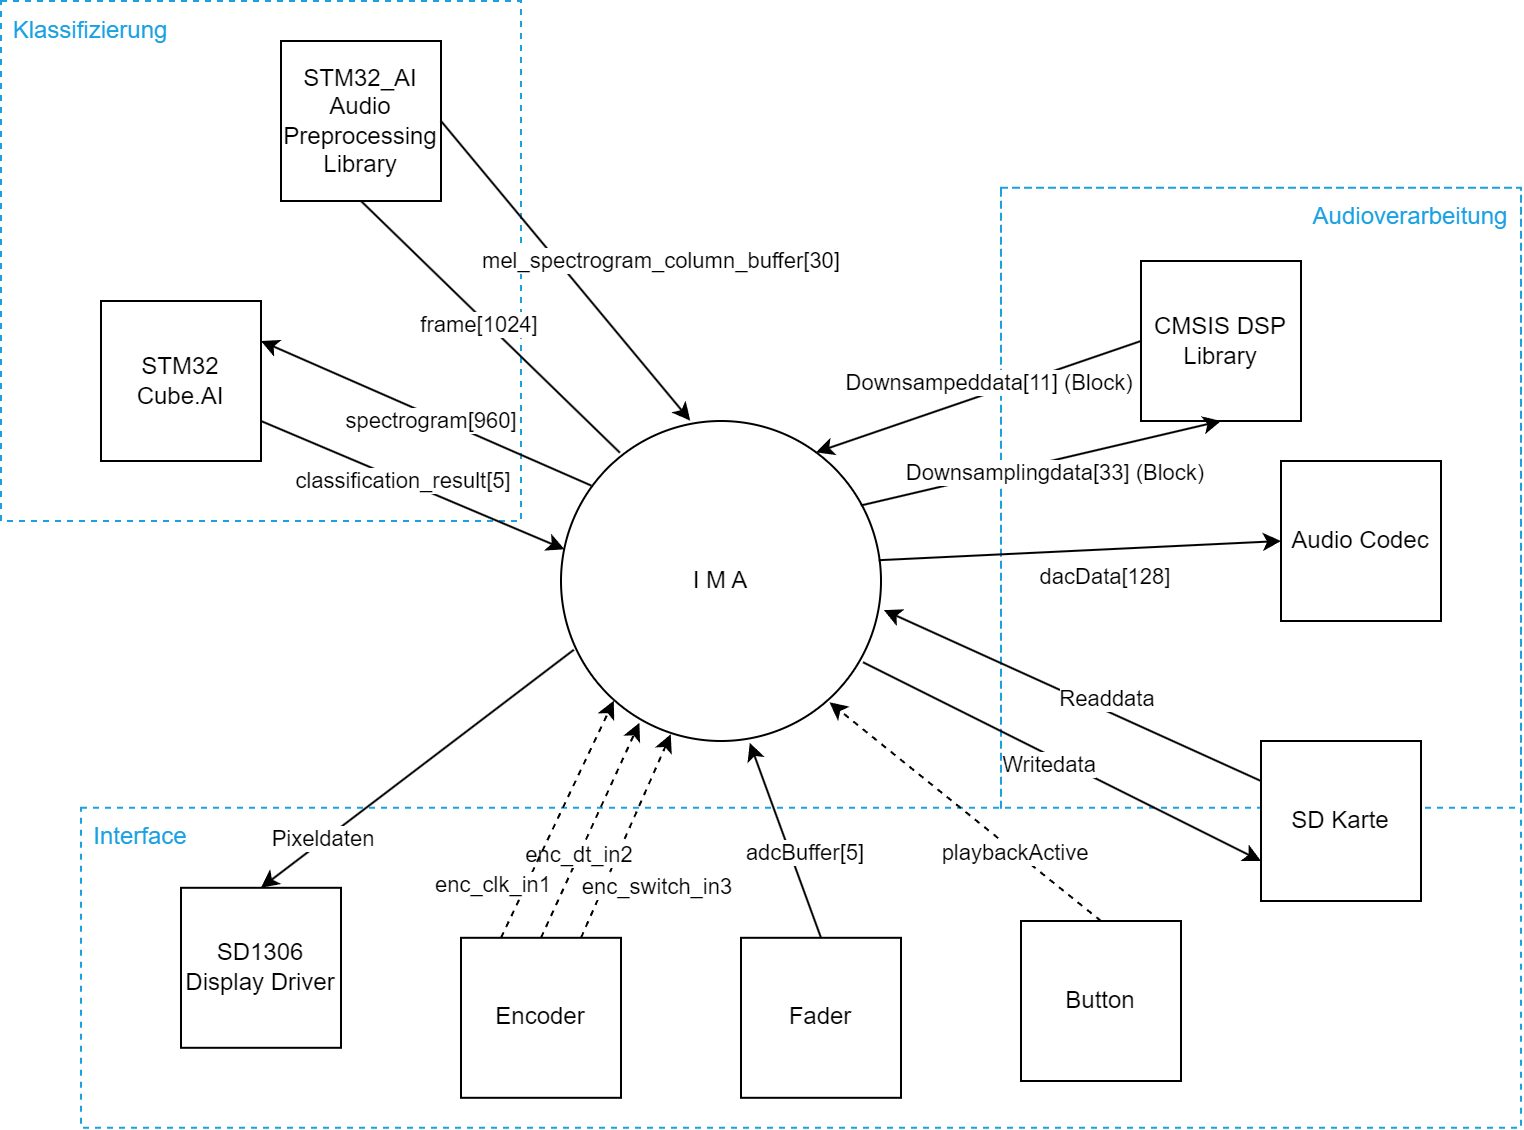
\includegraphics[width=0.8\textwidth]{images/04_spezifikation/kontextdiagramm_gesamt.drawio.png}
    	\caption{Kontextdiagramm des Gesamtsystems}
    	\label{fig:context_diagram_gesamt}
    \end{figure}
    
    %TODO: ausformulieren
    
    %TODO: Kontextdiagramme pro Untersystem
   
    
    \begin{figure}[H]
    	\centering
    	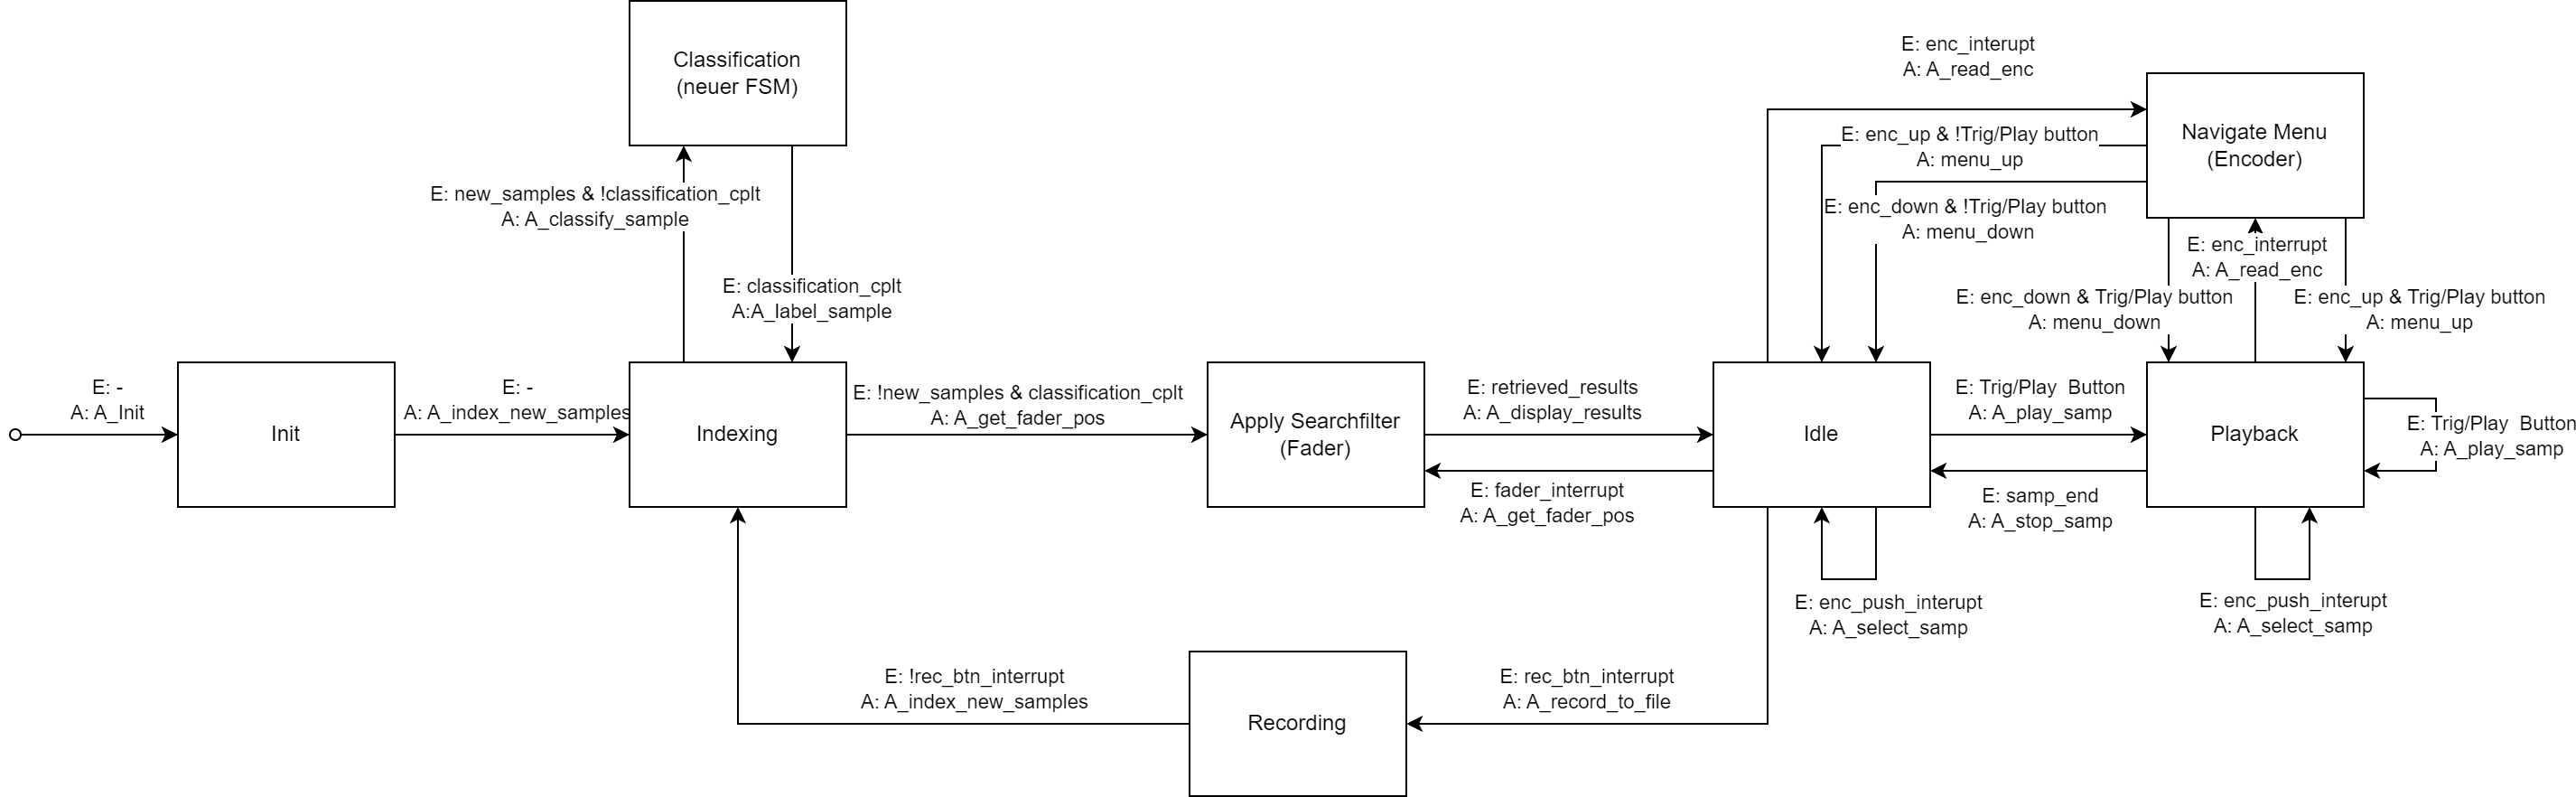
\includegraphics[width=1.0\textwidth]{images/04_spezifikation/fsm.drawio.png}
    	\caption{Zustandsautomat des Systems}
    	\label{fig:fsm}
    \end{figure}
    

\end{itemize}